\documentclass{article}
\usepackage[T1]{fontenc}
\usepackage{lmodern}
\usepackage{graphicx}
\usepackage{amsmath,amssymb}
\usepackage[a4paper,margin=2cm]{geometry}
\usepackage[absolute,overlay]{textpos}
\setlength{\TPHorizModule}{1mm}
\setlength{\TPVertModule}{1mm}
\usepackage[indonesian]{babel}
\usepackage{hyperref}
\setlength{\emergencystretch}{2em}
% unit: Halaman 57

\begin{document}

% === Halaman 57 (llm) ===

\begin{itemize}
    \item Contoh:
\end{itemize}

\vspace{5mm}

Kriptogram yang berulang adalah \textbf{LJV}

\begin{align*}
    \text{Jarak \textbf{LJV} ke-1 dengan \textbf{LJV} ke-2} &= 15 \\
    \text{Jarak \textbf{LJV} ke-2 dengan \textbf{LJV} ke-3} &= 15 \\
    \text{Jarak \textbf{LJV} ke-3 dengan \textbf{LJV} ke-4} &= 15 \\
    \text{Jarak \textbf{LJV} ke-4 dengan \textbf{LJV} ke-5} &= 10 \\
    \text{Jarak \textbf{LJV} ke-5 dengan \textbf{LJV} ke-6} &= 10
\end{align*}

Faktor pembagi $15 = \{3, 5, 15\}$

Faktor pembagi $10 = \{2, 5, 10\}$

Irisan kedua himpunan ini $= 5$. Jadi, panjang kunci diperkirakan $= 5$

% deskripsi: Teks kriptogram dengan penanda angka 1 sampai 6 di atas pola yang berulang 'LJV'.
% bbox normalisasi: [0.1010, 0.1430, 0.9180, 0.3440]
\begin{textblock*}{171.57mm}(21.21mm,42.47mm)
\noindent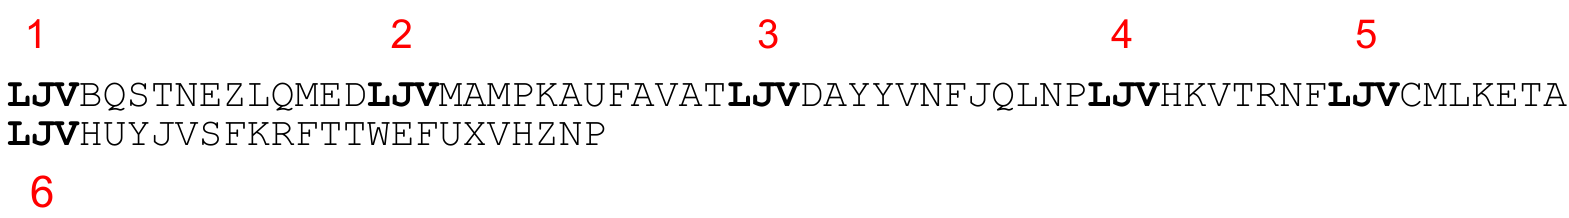
\includegraphics[width=171.57mm,height=59.70mm]{../../images/llm/page_057_img_01.png}%
\end{textblock*}

\end{document}
